\subsubsection{Package sequenziatore::client::ipresenter::iprocessowner::ilogic}
\begin{figure}[H] \centering 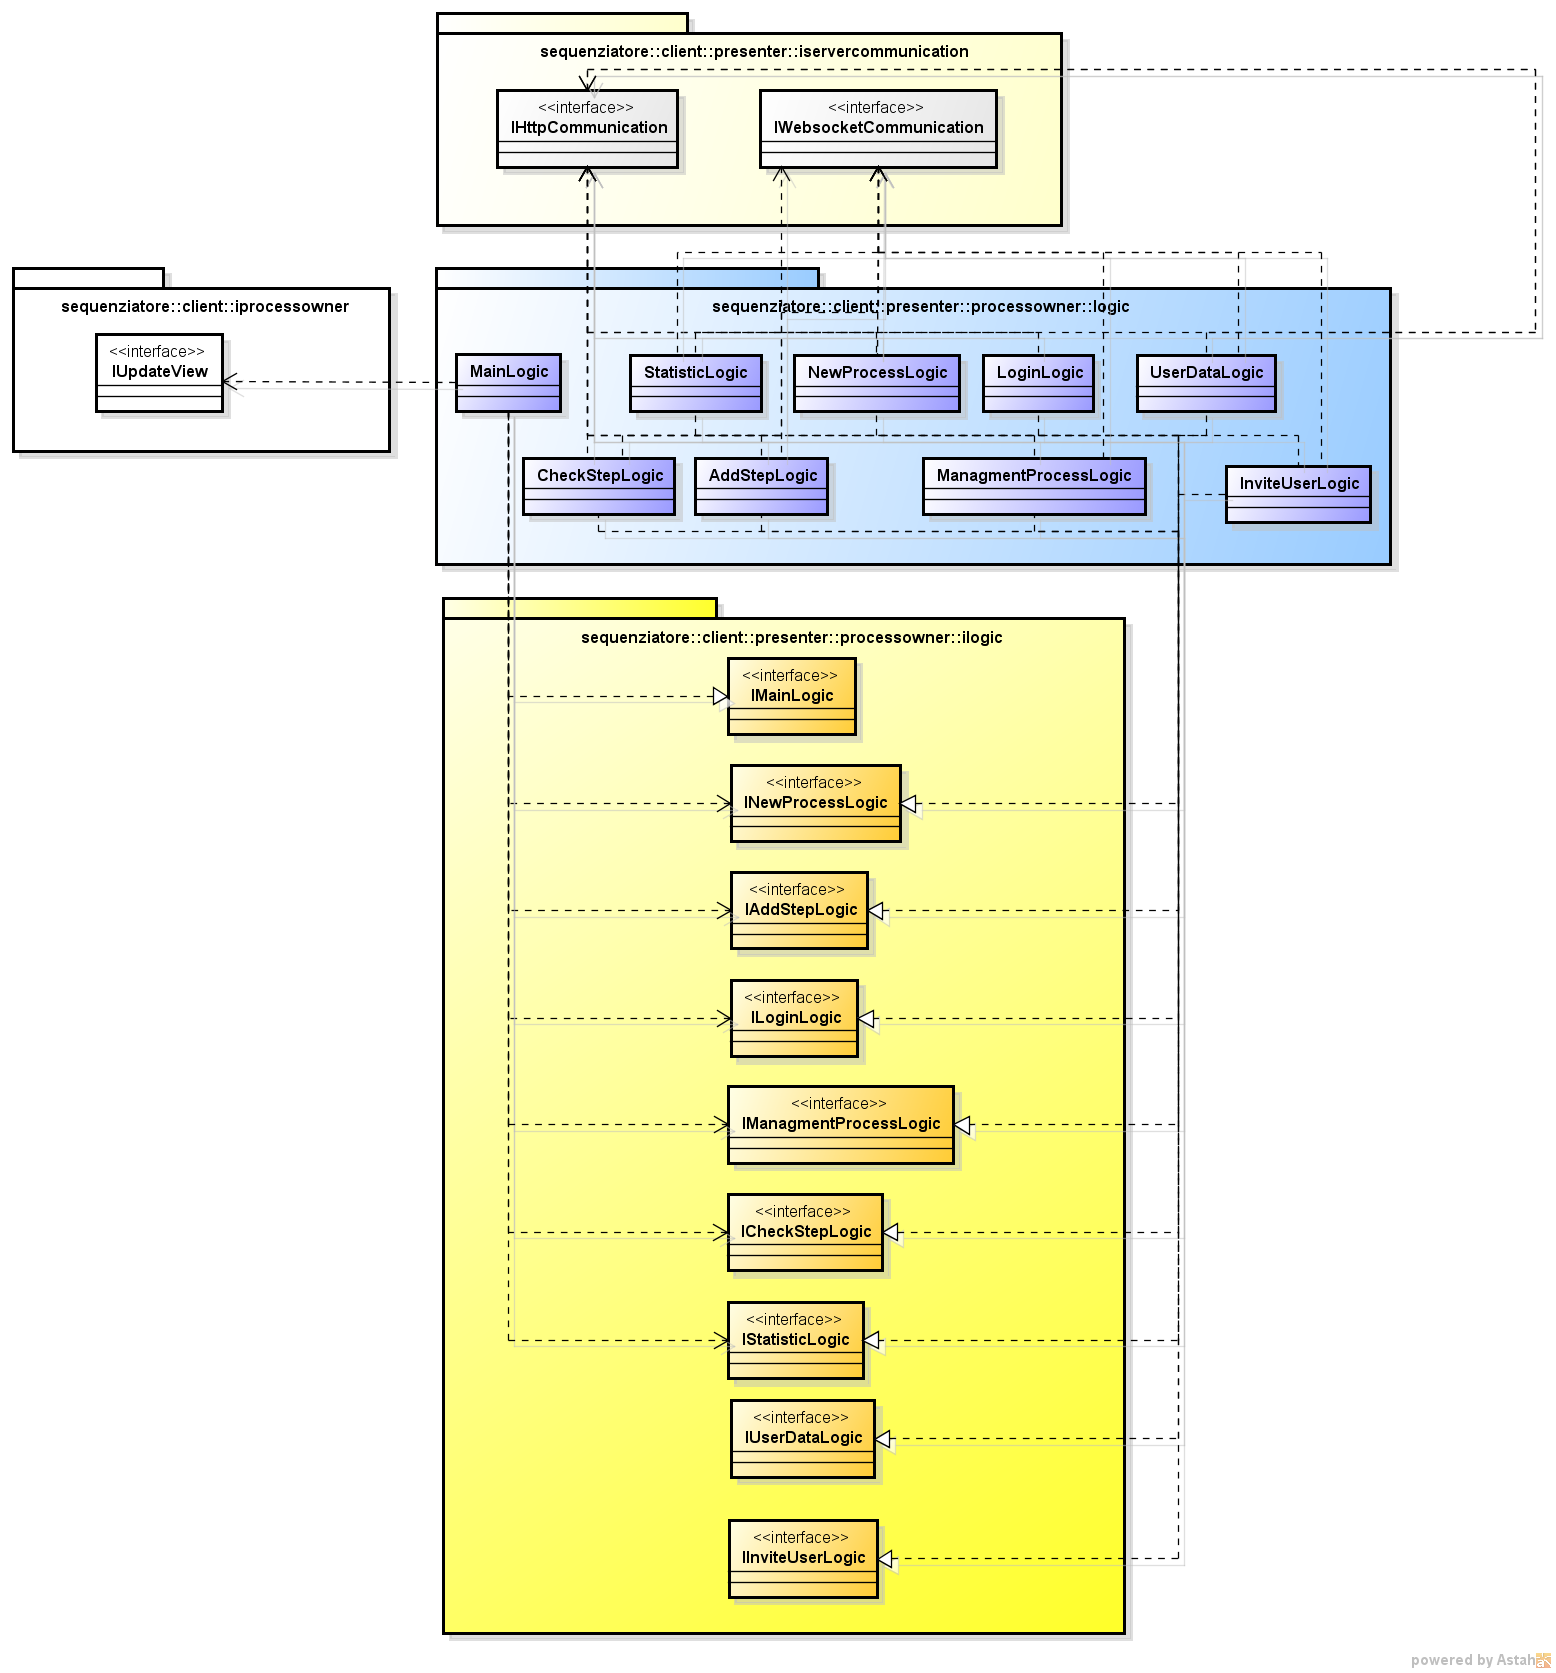
\includegraphics[width=%
\textwidth]
{./pack/presenter_PO.png} \caption{Diagramma presenter process owner}
\end{figure}
\paragraph{IIMainLogic}
\begin{itemize}
\item \textbf{Nome:} \texttt{IMainLogic};
\item \textbf{Package:} \texttt{\iLogicAdmin{}};
\item \textbf{Descrizione:} Interfaccia che permette di gestire gli eventi generati dalla componente \textit{View};
\end{itemize}

\paragraph{ILoginLogic}
\begin{itemize}
\item \textbf{Nome:} \texttt{ILoginLogic};
\item \textbf{Package:} \texttt{\iLogicAdmin{}};
\item \textbf{Descrizione:} Interfaccia che ha il compito di gestire le richieste di autenticazione e chiusura della sessione da parte dell'utente \textit{process owner}.
\end{itemize}

\paragraph{INewProcessLogic}
\begin{itemize}
\item \textbf{Nome:} \texttt{INewProcessLogic};
\item \textbf{Package:} \texttt{\iLogicAdmin{}};
\item \textbf{Descrizione:} Interfaccia che ha il compito di gestire la logica della definizione di un nuovo processo.
\end{itemize}


\paragraph{IAddStepLogic}
\begin{itemize}
\item \textbf{Nome:} \texttt{IAddStepLogic};
\item \textbf{Package:} \texttt{\iLogicAdmin{}};
\item \textbf{Descrizione:} Interfaccia che ha il compito di definire la logica di gestione dei passi di un processo.
\end{itemize}


\paragraph{IManagmentProcessLogic}

\begin{itemize}
\item \textbf{Nome:} \texttt{IManagmentProcessLogic};
\item \textbf{Package:} \texttt{\iLogicAdmin{}};
\item \textbf{Descrizione:} Interfaccia che ha il compito di gestire e accedere alle informazioni relative allo stato dei processi.
\end{itemize}


\paragraph{ICheckStepLogic}
\begin{itemize}
\item \textbf{Nome:} \texttt{ICheckStepLogic};
\item \textbf{Package:} \texttt{\iLogicAdmin{}};
\item \textbf{Descrizione:} Interfaccia che ha il compito di definire la logica del controllo di un passo che richiede intervento umano per essere approvato.
\end{itemize}


\paragraph{IStatisticLogic}
\begin{itemize}
\item \textbf{Nome:} \texttt{IStatisticLogic};
\item \textbf{Package:} \texttt{\iLogicAdmin{}};
\item \textbf{Descrizione:} Interfaccia che ha il compito di gestire l'accesso alle informazioni statistiche sui processi.
\end{itemize}


\paragraph{IUserDataLogic}
\begin{itemize}
\item \textbf{Nome:} \texttt{IUserDataLogic};
\item \textbf{Package:} \texttt{\iLogicAdmin{}};
\item \textbf{Descrizione:} Interfaccia che ha il compito gestire l'accesso alle informazioni sui passi superati dagli utenti.
\end{itemize}


\paragraph{IInviteUserLogic}
\begin{itemize}
\item \textbf{Nome:} \texttt{IInviteUserLogic};
\item \textbf{Package:} \texttt{\iLogicAdmin{}};
\item \textbf{Descrizione:} Interfaccia che ha il compito di gestire i permessi di iscrizione ad un processo degli utenti.
\end{itemize}
